\documentclass[11pt]{article}

\usepackage[margin=1in]{geometry}
\usepackage[T1]{fontenc}
\usepackage{lmodern}
\usepackage{microtype}
\usepackage{amsmath,amssymb}
\usepackage{booktabs}
\usepackage{graphicx}
\usepackage{xcolor}
\usepackage[numbers,sort&compress]{natbib}
\usepackage{tikz}
\usetikzlibrary{positioning,arrows.meta,fit,calc}
\usepackage{listings}
\usepackage[colorlinks=true,linkcolor=blue!60!black,citecolor=blue!60!black,urlcolor=blue!60!black]{hyperref}
\usepackage{cleveref}

\lstset{basicstyle=\ttfamily\footnotesize, columns=fullflexible, frame=single, framerule=0.3pt, rulecolor=\color{gray!50}, backgroundcolor=\color{gray!4}, showstringspaces=false, keepspaces=true}

\title{\textbf{HaloBlocks: A Registry-Based Library of Composable Attention,\\Mixture-of-Experts and Transformer Blocks for PyTorch}}
\author{B A NaveenKumar\\
\small Independent researcher\\
\small \url{https://github.com/basaanithanaveenkumar/HaloBlocks} \quad \texttt{pip install haloblocks}}
\date{}

\begin{document}
\maketitle

\begin{abstract}
Architecture research repeatedly re-implements the same layers, such as attention variants,
positional schemes and mixture-of-experts feed-forward networks, with slightly different
interfaces that make them hard to swap. \textbf{HaloBlocks} is a small PyTorch library,
published on PyPI, in which every component is a \texttt{Block} registered under its class
name. It can be created in three equivalent ways: directly
(\texttt{blocks.GroupedQueryAttention(...)}), by name (\texttt{hb.create("GroupedQueryAttention",
...)}), or from a nested configuration dictionary that can be stored as YAML or JSON. The
library ships 37 registered blocks: 24 attention blocks and helpers (scaled dot-product, multi-head,
multi-query, grouped-query, cross, gated, sliding-window with dilated and dynamic variants,
linear with three feature maps, multi-head latent attention with the absorption trick, and
QK-normalised output-gated ``Trinity'' attention); sinusoidal, learned, rotary and ALiBi
positions; RMSNorm; a configurable MLP; DeepSeek-style mixture-of-experts; transformer blocks
and decoders; and a flow-matching action decoder for vision--language--action models. A
\texttt{TransformerBlockBuilder} assembles a layer from \emph{any} registered attention,
cross-attention and feed-forward blocks with a declarative \texttt{operation\_order} (pre-norm,
post-norm, encoder--decoder), and \texttt{CompositeBlock} chains blocks into models. We describe
the design, report the test suite (71 tests, all passing) and measured sizes of example
compositions, and list the current interface inconsistencies found while writing this report.
\end{abstract}

\section{Introduction}

Transformer variants differ in small, local choices: how keys and values are shared across
heads~\cite{shazeer2019mqa,ainslie2023gqa}, compressed~\cite{deepseekv2}, restricted to a
window~\cite{beltagy2020longformer} or linearised~\cite{katharopoulos2020linear}; how positions
enter~\cite{su2021roformer,press2022alibi}; whether the output is gated~\cite{qiu2025gated}; and
whether the feed-forward network is dense or a mixture of
experts~\cite{shazeer2017outrageously,dai2024deepseekmoe}. Studying these choices requires
components that share an interface, so that swapping one for another is a one-line change.
Model-centric libraries~\cite{wolf2020transformers} optimise for faithful reproduction of
specific checkpoints rather than recombination.

HaloBlocks is built around three ideas:
\begin{enumerate}
  \item \textbf{One base class, one registry.} Every component subclasses \texttt{Block}
        (an \texttt{nn.Module}~\cite{paszke2019pytorch} with \texttt{forward(x, **kwargs)}) and
        is registered under its class name.
  \item \textbf{Three equivalent construction styles} (direct, by name, by config), so that
        interactive exploration and configuration-driven sweeps use the same objects.
  \item \textbf{Composition over inheritance.} Layers are assembled from parts by a builder
        and chained by a composite, instead of being subclassed for every combination.
\end{enumerate}

\section{Design}

\begin{figure}[t]
\centering
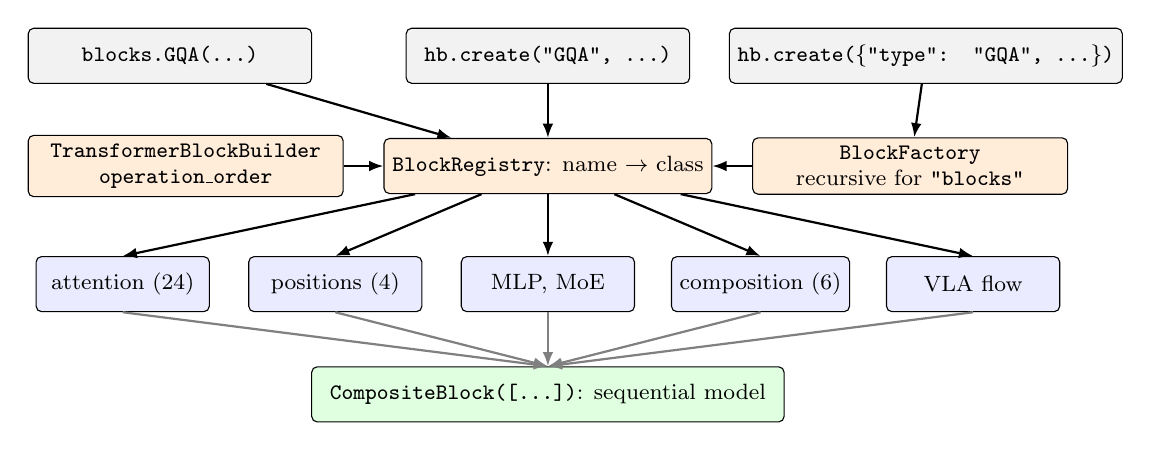
\begin{tikzpicture}[
  box/.style={draw, rounded corners=2pt, align=center, font=\footnotesize, minimum height=7mm, inner sep=3pt},
  api/.style={box, fill=gray!10, minimum width=36mm},
  core/.style={box, fill=orange!15, minimum width=40mm},
  blk/.style={box, fill=blue!8, minimum width=22mm},
  arr/.style={-{Latex[length=1.8mm]}, thick}
]
\node[api] (a1) at (-4.8,1.4) {\texttt{blocks.GQA(...)}};
\node[api] (a2) at (0,1.4) {\texttt{hb.create("GQA", ...)}};
\node[api] (a3) at (4.8,1.4) {\texttt{hb.create(\{"type": "GQA", ...\})}};
\node[core] (reg) at (0,0) {\texttt{BlockRegistry}: name $\to$ class};
\node[core] (fac) at (4.6,0) {\texttt{BlockFactory}\\recursive for \texttt{"blocks"}};
\node[core] (bld) at (-4.6,0) {\texttt{TransformerBlockBuilder}\\\texttt{operation\_order}};
\draw[arr] (a1) -- (reg); \draw[arr] (a2) -- (reg); \draw[arr] (a3) -- (fac); \draw[arr] (fac) -- (reg);
\draw[arr] (bld) -- (reg);
\foreach \n/\x/\lab in {att/-5.4/attention (24), pos/-2.7/positions (4), ffn/0/{MLP, MoE}, tr/2.7/composition (6), vla/5.4/VLA flow} {
  \node[blk] (\n) at (\x,-1.5) {\lab};
  \draw[arr] (reg) -- (\n.north);
}
\node[box, fill=green!12, minimum width=60mm] (comp) at (0,-2.9) {\texttt{CompositeBlock([...])}: sequential model};
\foreach \n in {att,pos,ffn,tr,vla} { \draw[arr, gray] (\n.south) -- (comp.north); }
\end{tikzpicture}
\caption{HaloBlocks API (GQA abbreviates \texttt{GroupedQueryAttention}). Three construction styles resolve through one registry. Builder and
composite blocks assemble registered components into layers and models. The numbers
count registry entries, including helper classes such as feature maps and head sub-blocks.}
\label{fig:api}
\end{figure}

\paragraph{Block and registry.} \texttt{Block} fixes the call signature \texttt{forward(x, **kwargs)}.
Extra inputs such as masks or context are keyword arguments, so containers can forward them
without knowing which children use them. \texttt{BlockRegistry.register()} stores the class
under its name (optionally an alias). \texttt{BlockFactory.create} accepts a name plus
keyword arguments or a dictionary with a \texttt{type} key, and recursively builds any nested
\texttt{"blocks"} list, so a whole model is one JSON- or YAML-serialisable object (\cref{fig:api}).

\paragraph{Builder.} \texttt{TransformerBlockBuilder} takes an attention, an optional
cross-attention and a feed-forward specification, each of which can be \texttt{None}
(default), a registry name, a config dictionary or an already-built block. It also takes a
norm type (LayerNorm~\cite{xiong2020layer} or RMSNorm~\cite{zhang2019rmsnorm}) and an
\texttt{operation\_order}: a tuple of sublayers, each a tuple of operations drawn from
\{\texttt{norm}, \texttt{self\_attn}, \texttt{cross\_attn}, \texttt{ffn}\}. Named presets cover
pre-norm \texttt{((norm, self\_attn), (norm, ffn))}, post-norm, and their encoder--decoder
versions with cross-attention. A flat order is grouped automatically at each compute
operation. The builder injects \texttt{emb\_dim} only into blocks whose constructor accepts
it. \texttt{StackedTransformerBlock} repeats a built layer $N$ times.

\begin{lstlisting}[language=Python, caption={A GQA + MoE layer and a four-layer Trinity model built from configs.}, label=lst:ex]
layer = hb.create("TransformerBlockBuilder", emb_dim=256, norm="rmsnorm",
    attn={"type": "GroupedQueryAttention", "num_heads": 8, "num_kv_heads": 2},
    ffn={"type": "DeepseekMoE", "emb_dim": 256, "hid_dim": 512,
         "num_router_exprts": 8, "best_k": 2, "num_shared_exprts": 1})
model = hb.create({"type": "CompositeBlock", "blocks": [
    {"type": "SinusoidalPositionalEmbedding", "emb_dim": 256, "max_len": 128},
    {"type": "StackedTransformerBlock", "emb_dim": 256, "num_layers": 4,
     "attn": {"type": "TrinityAttention", "num_heads": 8}, "norm": "rmsnorm"}]})
\end{lstlisting}

\section{Block Catalogue}

\begin{table}[t]
\centering
\caption{Registered blocks (37 registry entries).}
\label{tab:catalogue}
\small
\begin{tabular}{lp{10.4cm}}
\toprule
Family & Blocks \\
\midrule
Attention & ScaledDotProduct, Self, Head, MultiHead~\cite{vaswani2017attention}, MultiQuery~\cite{shazeer2019mqa}, GroupedQuery~\cite{ainslie2023gqa}, Cross, HeadCross, MultiHeadCross, Gated, GatedWithMask, GatedCross~\cite{qiu2025gated}, SlidingWindow, DilatedSlidingWindow, DynamicSlidingWindow~\cite{beltagy2020longformer}, Linear, LinearWithRoPE, LinearCross with ELU/ReLU/Exp feature maps~\cite{katharopoulos2020linear}, MultiHeadLatent~\cite{deepseekv2}, Trinity, TrinityCross \\
Positions & Sinusoidal~\cite{vaswani2017attention}, Learned, Rotary~\cite{su2021roformer}, ALiBi~\cite{press2022alibi} \\
Norm / FFN & RMSNorm~\cite{zhang2019rmsnorm}, MLP, DeepseekMoE~\cite{dai2024deepseekmoe} \\
Composition & CompositeBlock, TransformerBlock, DecoderTransformer, TransformerBlockBuilder, StackedTransformerBlock(s) \\
VLA & FlowActionDecoder~\cite{lipman2023flow,black2024pi0} \\
\bottomrule
\end{tabular}
\end{table}

\Cref{tab:catalogue} lists the registered blocks. A few deserve detail.

\paragraph{Multi-head latent attention.} Keys and values are down-projected to a shared latent of
width $d_c$ (default $d/4$) and up-projected per head, following DeepSeek-V2~\cite{deepseekv2}.
With the \emph{absorption trick}, queries are multiplied by the key up-projection so that
attention scores are computed directly against the compressed latent,
$q^\top (W^{UK} c) = (W^{UK\top} q)^\top c$, which avoids materialising full keys. This is the
basis of MLA's small KV cache.

\paragraph{Gated and Trinity attention.} \texttt{GatedAttention} multiplies the attention output
by a sigmoid gate computed from the input, $o = W_o\big(\sigma(W_g x + b_g)\odot \mathrm{Attn}(x)\big)$,
with an optional negative bias initialisation that starts the gate mostly closed. Output
gating of this kind adds non-linearity and sparsity and removes attention sinks~\cite{qiu2025gated}.
\texttt{TrinityAttention} is the same gated form with per-head RMSNorm on queries and keys
(QK-norm~\cite{henry2020qknorm}) enabled by default, and a cross-attention counterpart.

\paragraph{Linear and windowed attention.} \texttt{LinearAttention} replaces the softmax kernel with
a positive feature map $\phi$ (ELU$+1$, ReLU or exponential), giving cost linear in sequence
length~\cite{katharopoulos2020linear}. A RoPE variant adds rotary position embeddings to
linear attention. Sliding-window attention restricts each query to a local window, with dilated
and dynamically sized variants.

\paragraph{DeepSeek MoE and flow decoder.} \texttt{DeepseekMoE} combines always-active shared SwiGLU
experts~\cite{shazeer2020glu} with routed experts selected by a noisy top-$k$
router~\cite{shazeer2017outrageously,dai2024deepseekmoe}. \texttt{FlowActionDecoder} predicts the
velocity field $v_\theta(x_t,t,c)$ of a flattened action chunk from the noisy chunk, a
sinusoidal time embedding and an observation embedding. It is trained with conditional flow
matching~\cite{lipman2023flow} and used as a VLA action head~\cite{black2024pi0}.

\section{Validation}

The test suite covers the core (registry, factory, composite, builder and its operation
orders), every attention family (shapes, masks, divisibility errors), positional embeddings,
norms, the MLP, and the three construction styles for each block. All 71 tests pass (PyTorch
2.14, Python 3.12, CPU). Example sizes, measured: the GQA + MoE layer in \cref{lst:ex} has
3.71M parameters, and the four-layer Trinity model has 3.42M. Both map $(2,16,256)$ inputs
to $(2,16,256)$ outputs. CI runs the tests on pushes and pull requests to \texttt{main}, and a merged release pull request
tags the version and publishes it to PyPI automatically.

\section{Known Inconsistencies}

While writing this report we found three places where the documentation and interfaces
disagree. We list them for users of the current release (v0.1.3). (i)~The README describes
TrinityAttention as combining local, global and linear attention, but the implementation is
QK-normalised softmax attention with a sigmoid output gate, as described above.
(ii)~Passing \texttt{ffn="DeepseekMoE"} as a string with \texttt{ffn\_kwargs} to the builder fails,
because default MLP arguments are merged into the MoE constructor. The dictionary form in
\cref{lst:ex} works. (iii)~The README's build badge references a workflow name that does not
exist.

\section{Conclusion}

HaloBlocks shows that a single base class, a name registry and two composition primitives
are enough to make a wide range of modern attention and MoE designs interchangeable. That
turns architecture comparisons into configuration edits, while every block remains plain
PyTorch.

\bibliographystyle{plainnat}
\bibliography{references}

\end{document}
